\documentclass{standalone}

%----------------------------------------------------------------------------------------------%
%                                 Packages and basic declarations
%----------------------------------------------------------------------------------------------%

\usepackage[utf8]{inputenc}
\usepackage{pgfplots}
\usepackage{tikz}


%----------------------------------------------------------------------------------------------%
%----------------------------------------------------------------------------------------------%
%                                            DOCUMENT STARTS
%----------------------------------------------------------------------------------------------%
%----------------------------------------------------------------------------------------------%

\begin{document}


%Tikz picture starts%

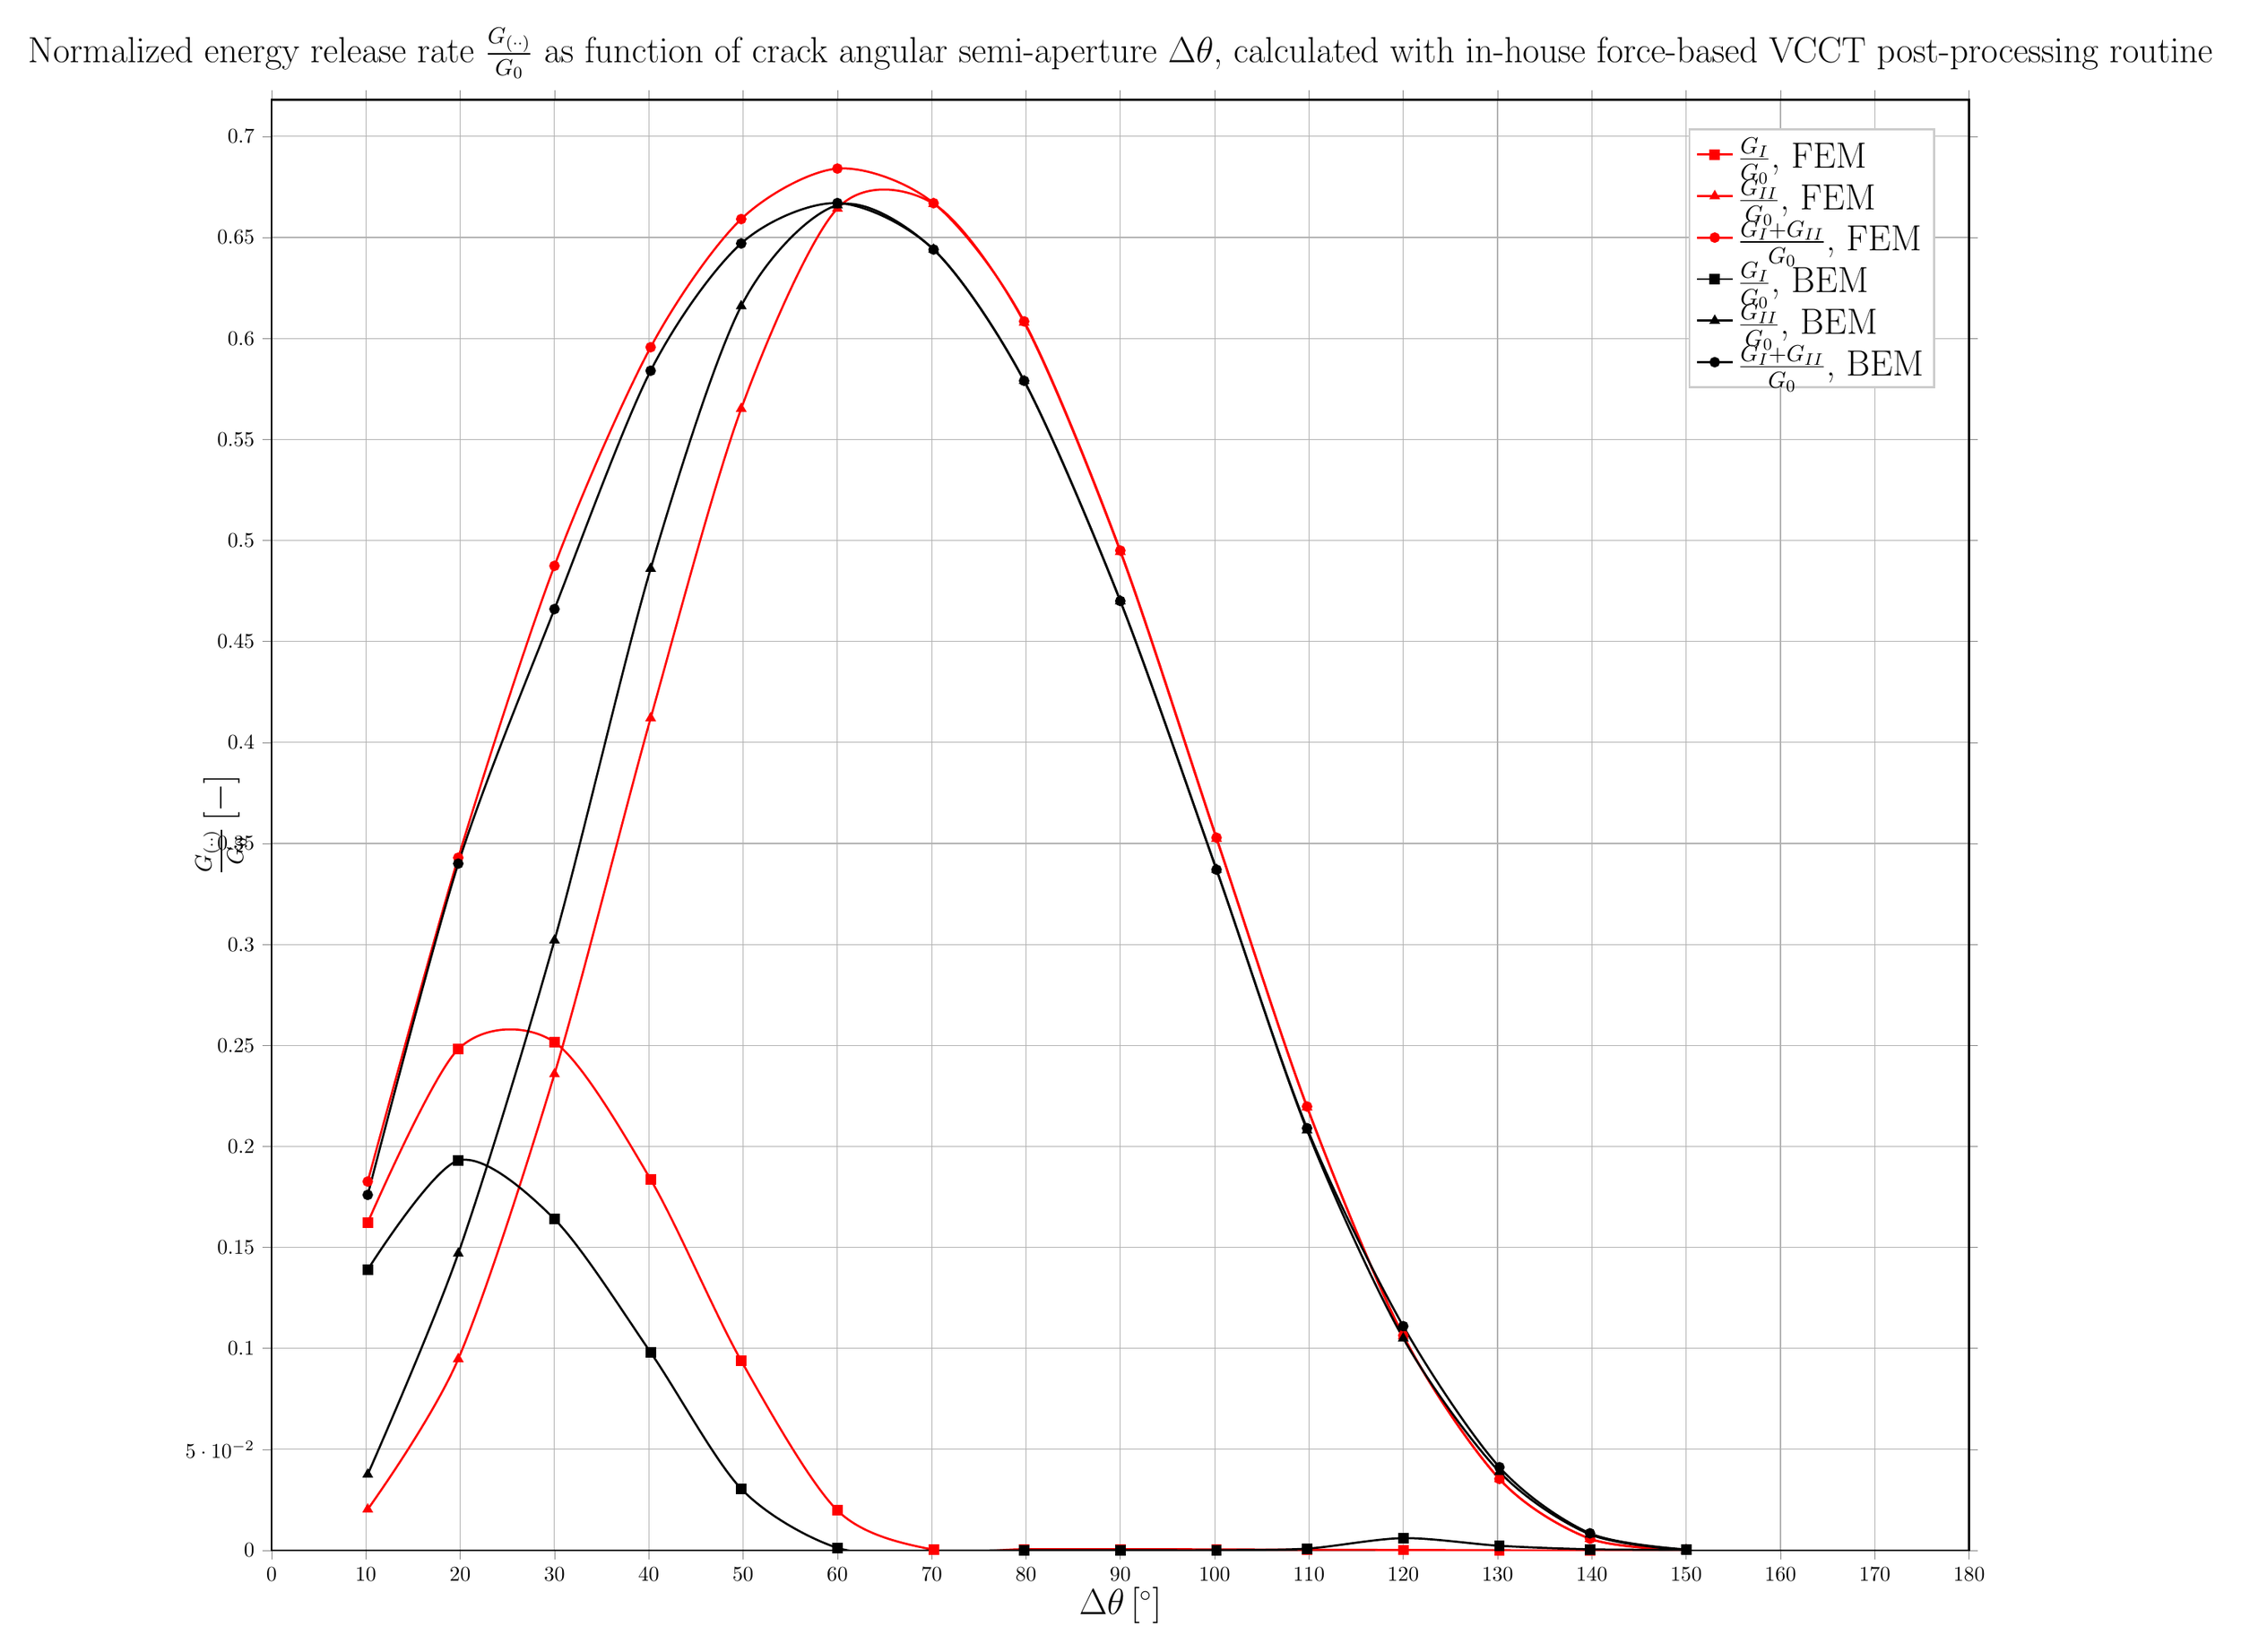
\begin{tikzpicture}

%Tikz axis starts%

\begin{axis}[width=30cm,
title={Normalized energy release rate $\frac{G_{\left(\cdot\cdot\right)}}{G_{0}}$ as function of crack angular semi-aperture  $\Delta\theta$, calculated with in-house force-based VCCT post-processing routine},
title style={font=\fontsize{16}{8}\selectfont},
xlabel style={at={(axis description cs:0.5,-0.02)},anchor=north,font=\fontsize{16}{8}\selectfont},
ylabel style={at={(axis description cs:-0.01,.5)},anchor=south,font=\fontsize{16}{8}\selectfont},
xlabel={$\Delta\theta\left[^{\circ}\right]$},ylabel={$\frac{G_{\left(\cdot\cdot\right)}}{G_{0}}\left[-\right]$},
xmin=0.0,
xmax=180.0,
ymin=0.0,
ymax=0.718284770048,
tick align=outside,
tick label style={font=\normalsize},
xtick={0.0,10.0,20.0,30.0,40.0,50.0,60.0,70.0,80.0,90.0,100.0,110.0,120.0,130.0,140.0,150.0,160.0,170.0,180.0},
xmajorgrids,
x grid style={lightgray!92.026143790849673!black},
ymajorgrids,
y grid style={lightgray!92.026143790849673!black},
line width=0.35mm,
legend style={draw=white!80.0!black,font=\fontsize{16}{12}\selectfont},
legend entries={{$\frac{G_{I}}{G_{0}}$, FEM},{$\frac{G_{II}}{G_{0}}$, FEM},{$\frac{G_{I}+G_{II}}{G_{0}}$, FEM},{$\frac{G_{I}}{G_{0}}$, BEM},{$\frac{G_{II}}{G_{0}}$, BEM},{$\frac{G_{I}+G_{II}}{G_{0}}$, BEM}},
legend cell align={left}
]

\addplot[red,smooth,mark=square*]
table{
10.1996888272 0.162281406164
19.800125885 0.248168118164
29.9998676461 0.251594978398
40.1999526243 0.183605714666
49.8000464651 0.0938871359878
60.0001314432 0.019782622213
70.1998714969 0.000296769394868
79.8003102622 0.000588479972312
90.0000025045 0.000571584474209
100.199687917 0.000514299579946
109.800126682 0.000336071847341
119.999866736 0.0002255944052
130.199948299 8.24465570517e-05
139.800052385 1.20050610992e-05
150.000133948 0.000380138337889
};

\addplot[red,smooth,mark=triangle*]
table{
10.1996888272 0.0203179543988
19.800125885 0.0947574169364
29.9998676461 0.23580338738
40.1999526243 0.412029716888
49.8000464651 0.565189448937
60.0001314432 0.664298111166
70.1998714969 0.66665115423
79.8003102622 0.607845191927
90.0000025045 0.494409077202
100.199687917 0.352310947309
109.800126682 0.219400439324
119.999866736 0.106152095457
130.199948299 0.0352879244229
139.800052385 0.00578358824137
150.000133948 0.000107528058795
};

\addplot[red,smooth,mark=*]
table{
10.1996888272 0.182599360562
19.800125885 0.3429255351
29.9998676461 0.487398365779
40.1999526243 0.595635431554
49.8000464651 0.659076584925
60.0001314432 0.684080733379
70.1998714969 0.666947923625
79.8003102622 0.6084336719
90.0000025045 0.494980661676
100.199687917 0.352825246889
109.800126682 0.219736511171
119.999866736 0.106377689862
130.199948299 0.0353703709799
139.800052385 0.00579559330247
150.000133948 0.000487666396684
};

\addplot[black,smooth,mark=square*]
table{
10.1996888272 0.139
19.800125885 0.193
29.9998676461 0.164
40.1999526243 0.098
49.8000464651 0.0305
60.0001314432 0.00127
70.1998714969 -4.79e-05
79.8003102622 6.85e-05
90.0000025045 0.000112
100.199687917 0.000112
109.800126682 0.000895
119.999866736 0.00607
130.199948299 0.00229
139.800052385 0.000552
150.000133948 0.000306
};

\addplot[black,smooth,mark=triangle*]
table{
10.1996888272 0.0376
19.800125885 0.147
29.9998676461 0.302
40.1999526243 0.486
49.8000464651 0.616
60.0001314432 0.666
70.1998714969 0.644
79.8003102622 0.579
90.0000025045 0.47
100.199687917 0.337
109.800126682 0.208
119.999866736 0.105
130.199948299 0.0389
139.800052385 0.00792
150.000133948 0.000165
};

\addplot[black,smooth,mark=*]
table{
10.1996888272 0.176
19.800125885 0.34
29.9998676461 0.466
40.1999526243 0.584
49.8000464651 0.647
60.0001314432 0.667
70.1998714969 0.644
79.8003102622 0.579
90.0000025045 0.47
100.199687917 0.337
109.800126682 0.209
119.999866736 0.111
130.199948299 0.0412
139.800052385 0.00847
150.000133948 0.000471
};

\end{axis}
%Tikz axis ends%


\end{tikzpicture}
%Tikz picture ends%


\end{document}

%----------------------------------------------------------------------------------------------%
%----------------------------------------------------------------------------------------------%
%                                            DOCUMENT ENDS
%----------------------------------------------------------------------------------------------%
%----------------------------------------------------------------------------------------------%

